% generated by GAPDoc2LaTeX from XML source (Frank Luebeck)
\documentclass[a4paper,11pt]{report}

\usepackage[top=37mm,bottom=37mm,left=27mm,right=27mm]{geometry}
\sloppy
\pagestyle{myheadings}
\usepackage{amssymb}
\usepackage[latin1]{inputenc}
\usepackage{makeidx}
\makeindex
\usepackage{color}
\definecolor{FireBrick}{rgb}{0.5812,0.0074,0.0083}
\definecolor{RoyalBlue}{rgb}{0.0236,0.0894,0.6179}
\definecolor{RoyalGreen}{rgb}{0.0236,0.6179,0.0894}
\definecolor{RoyalRed}{rgb}{0.6179,0.0236,0.0894}
\definecolor{LightBlue}{rgb}{0.8544,0.9511,1.0000}
\definecolor{Black}{rgb}{0.0,0.0,0.0}

\definecolor{linkColor}{rgb}{0.0,0.0,0.554}
\definecolor{citeColor}{rgb}{0.0,0.0,0.554}
\definecolor{fileColor}{rgb}{0.0,0.0,0.554}
\definecolor{urlColor}{rgb}{0.0,0.0,0.554}
\definecolor{promptColor}{rgb}{0.0,0.0,0.589}
\definecolor{brkpromptColor}{rgb}{0.589,0.0,0.0}
\definecolor{gapinputColor}{rgb}{0.589,0.0,0.0}
\definecolor{gapoutputColor}{rgb}{0.0,0.0,0.0}

%%  for a long time these were red and blue by default,
%%  now black, but keep variables to overwrite
\definecolor{FuncColor}{rgb}{0.0,0.0,0.0}
%% strange name because of pdflatex bug:
\definecolor{Chapter }{rgb}{0.0,0.0,0.0}
\definecolor{DarkOlive}{rgb}{0.1047,0.2412,0.0064}


\usepackage{fancyvrb}

\usepackage{mathptmx,helvet}
\usepackage[T1]{fontenc}
\usepackage{textcomp}


\usepackage[
            pdftex=true,
            bookmarks=true,        
            a4paper=true,
            pdftitle={Written with GAPDoc},
            pdfcreator={LaTeX with hyperref package / GAPDoc},
            colorlinks=true,
            backref=page,
            breaklinks=true,
            linkcolor=linkColor,
            citecolor=citeColor,
            filecolor=fileColor,
            urlcolor=urlColor,
            pdfpagemode={UseNone}, 
           ]{hyperref}

\newcommand{\maintitlesize}{\fontsize{36}{38}\selectfont}

% write page numbers to a .pnr log file for online help
\newwrite\pagenrlog
\immediate\openout\pagenrlog =\jobname.pnr
\immediate\write\pagenrlog{PAGENRS := [}
\newcommand{\logpage}[1]{\protect\write\pagenrlog{#1, \thepage,}}
%% were never documented, give conflicts with some additional packages

\newcommand{\GAP}{\textsf{GAP}}

%% nicer description environments, allows long labels
\usepackage{enumitem}
\setdescription{style=nextline}

%% depth of toc
\setcounter{tocdepth}{1}



\usepackage[pdftex]{graphicx}

%% command for ColorPrompt style examples
\newcommand{\gapprompt}[1]{\color{promptColor}{\bfseries #1}}
\newcommand{\gapbrkprompt}[1]{\color{brkpromptColor}{\bfseries #1}}
\newcommand{\gapinput}[1]{\color{gapinputColor}{#1}}


\begin{document}

\logpage{[ 0, 0, 0 ]}
\begin{titlepage}
\mbox{}\vfill

\begin{center}{\maintitlesize \textbf{The \textsf{GAP} 4 Development Manual\\
\mbox{}}}\\
\vfill

\hypersetup{pdftitle={The \textsf{GAP} 4 Development Manual}}
\markright{\scriptsize \mbox{}\hfill The \textsf{GAP} 4 Development Manual \hfill\mbox{}}
{\Huge \textbf{Administrating the \textsf{GAP} Project\\
\mbox{}}}\\
\vfill

{2015\mbox{}}\\[1cm]
\mbox{}\\[2cm]
{\Large \textbf{\strut The \textsf{GAP} Group    \strut\mbox{}}}\\
\hypersetup{pdfauthor={The \textsf{GAP} Group   }}
\end{center}\vfill

\mbox{}\\
{\mbox{}\\
\small \noindent \textbf{The \textsf{GAP} Group   }  Email: \href{mailto://support@gap-system.org} {\texttt{support@gap\texttt{\symbol{45}}system.org}}\\
  Homepage: \href{https://www.gap-system.org} {\texttt{https://www.gap\texttt{\symbol{45}}system.org}}}\\
\end{titlepage}

\newpage\setcounter{page}{2}
{\small 
\section*{Abstract}
\logpage{[ 0, 0, 1 ]}
 In this \emph{development manual} we collect documentation of various tasks needed for the further development,
maintenance and distribution of \textsf{GAP}. 

 Some sections provide practical howto's and check lists for tasks like, e.g.:
committing changes, testing, wrapping archives, compiling documentation. 

 Other sections document certain conventions which are followed by the active
members of The \textsf{GAP} Group. Some examples: there are several mailing lists which are used for
different purposes; there is a mechanism how larger changes to the \textsf{GAP} system should be announced and discussed among the developers before they are
committed, called \emph{proposals}; there is a concept of \emph{modules} where parts of the \textsf{GAP} system are assigned to specified maintainers. \mbox{}}\\[1cm]
{\small 
\section*{Copyright}
\logpage{[ 0, 0, 2 ]}
 {\copyright} (2005\texttt{\symbol{45}}this year) The \textsf{GAP} Group\mbox{}}\\[1cm]
\newpage

\def\contentsname{Contents\logpage{[ 0, 0, 3 ]}}

\tableofcontents
\newpage

  
\chapter{\textcolor{Chapter }{Structure of the \textsf{GAP} distribution}}\label{Chap-Structure}
\logpage{[ 1, 0, 0 ]}
\hyperdef{L}{X7A2465B67D8E59B6}{}
{
  Here is a short overview of the structure of the \textsf{GAP} distribution and repository. 
\section{\textcolor{Chapter }{Kernel, library, documentation, package interface, development part}}\label{Sect-Parts}
\logpage{[ 1, 1, 0 ]}
\hyperdef{L}{X7B27E71B7AA26F31}{}
{
  ... }

 
\section{\textcolor{Chapter }{The directories of the \textsf{GAP} distribution and repository}}\label{Sect-GapDirs}
\logpage{[ 1, 2, 0 ]}
\hyperdef{L}{X7C387B4C84A76B5B}{}
{
  ... }

 }

  
\chapter{\textcolor{Chapter }{The \textsf{GAP} kernel programming}}\label{Chap-Kernel}
\logpage{[ 2, 0, 0 ]}
\hyperdef{L}{X810D56CE7BC6031F}{}
{
  
\section{\textcolor{Chapter }{Overview of the \textsf{GAP} kernel}}\label{Sect-Kinds}
\logpage{[ 2, 1, 0 ]}
\hyperdef{L}{X8071E6CA7A9CF5DF}{}
{
  The \textsf{GAP} kernel consists of more than 150000 lines of \textsf{C} code that: 
\begin{itemize}
\item provides the run\texttt{\symbol{45}}time environment and user interface;
\item interprets the \textsf{GAP} language;
\item performs arithmetic operations with basic types of objects;
\item speeds up some time\texttt{\symbol{45}}critical operations.
\end{itemize}
 The \textsf{GAP} kernel code mainly falls into the four main categories: 
\begin{enumerate}
\item Implementations for basic data types and structures (integers, permutations,
finite field elements, etc.), which has to be in the kernel for the maximal
efficiency.
\item Low level access methods for data objects (lists, ranges, records, etc.).
\item Various methods for handling complex \textsf{GAP} objects in component and positional representation from the kernel.
\item \textsf{GAP} foundations such as \textsf{GAP} language, garbage collector (in what follows \texttt{\symbol{45}} GC), etc.
\end{enumerate}
 The \textsf{GAP} kernel programming has four levels of sofistication: 
\begin{enumerate}
\item The simplest form of kernel programming is to add new kernel functions for
manipulating existing data types.
\item Using the "data object" type to add new binary data structures to the kernel.
\item Adding new basic (primitive) data types, such as, for example, \emph{Floats}.
\item Modifying the foundations, for example, changing the syntax of the \textsf{GAP} language.
\end{enumerate}
 We will cover only first two levels here, while adding new basic data types or
modifying the foundations are outside the scope of this manual. }

 
\section{\textcolor{Chapter }{"Hello World" example}}\label{Sect-HelloWorld}
\logpage{[ 2, 2, 0 ]}
\hyperdef{L}{X7F9BD7A37B142C23}{}
{
  On the \textsf{GAP} level, the kernel functionality may be accessed via kernel functions. You can
recognise such functions because they will be displayed as compiled code in
the \textsf{GAP} session: 
\begin{Verbatim}[commandchars=!@|,fontsize=\small,frame=single,label=]
  
  !gapprompt@gap>| !gapinput@Display(TYPE_OBJ);|
  function ( obj )
      <<kernel code>> from src/objects.c:TYPE_OBJ
  end
  
\end{Verbatim}
 Let us demonstrate how to add a kernel function that will print "Hello
World!". Such function has no arguments and returns nothing. To add it, we
need to perform three basic steps: 
\begin{enumerate}
\item  Create the \textsf{C} handler, adding to the file \texttt{string.c} (this file contains the functions which mainly deal with strings) the \textsf{C} code doing the actual job (see the function \texttt{Pr} to print formatted output in the file \texttt{scanner.c} ): 
\begin{Verbatim}[commandchars=@|A,fontsize=\small,frame=single,label=]
  
  static Obj FuncHELLO_WORLD(Obj self)
  {
      Pr("Hello World!\n", 0, 0);
      return 0;
  }
  
\end{Verbatim}
 This code should be placed somewhere in the file \texttt{string.c} before specifying \texttt{GvarFuncs}. 
\item  In the same file \texttt{string.c} find the list of functions to export called \texttt{GvarFuncs} and add to this list a table entry for \texttt{HELLO{\textunderscore}WORLD} 
\begin{Verbatim}[commandchars=!@|,fontsize=\small,frame=single,label=]
  
  GVAR_FUNC_0ARGS(HELLO_WORLD),
  
\end{Verbatim}
 containing respectively the string specifying the name of the function at the \textsf{GAP} level, the number of arguments, the string with the description of arguments,
corresponding \textsf{C} handler and the string (``cookie'') specifying the location of this handler (see definition of the structure \texttt{StructGVarFunc} in the file \texttt{system.h} ). 
\item  Compile the \textsf{GAP} kernel, and now \texttt{HELLO{\textunderscore}WORLD();} will work. 
\begin{Verbatim}[commandchars=@|A,fontsize=\small,frame=single,label=Example]
  
  @gapprompt|gap>A @gapinput|HELLO_WORLD();A
  Hello World!
  
\end{Verbatim}
 
\end{enumerate}
 }

 
\section{\textcolor{Chapter }{Structure of the \textsf{GAP} kernel}}\label{Sect-BigPicture}
\logpage{[ 2, 3, 0 ]}
\hyperdef{L}{X78D70F927B947A2C}{}
{
  The following picture is based on the scheme that Martin Sch{\"o}nert drew in
1995 and displays the structure of the \textsf{GAP} kernel: 
\centerline{\resizebox{130mm}{!}{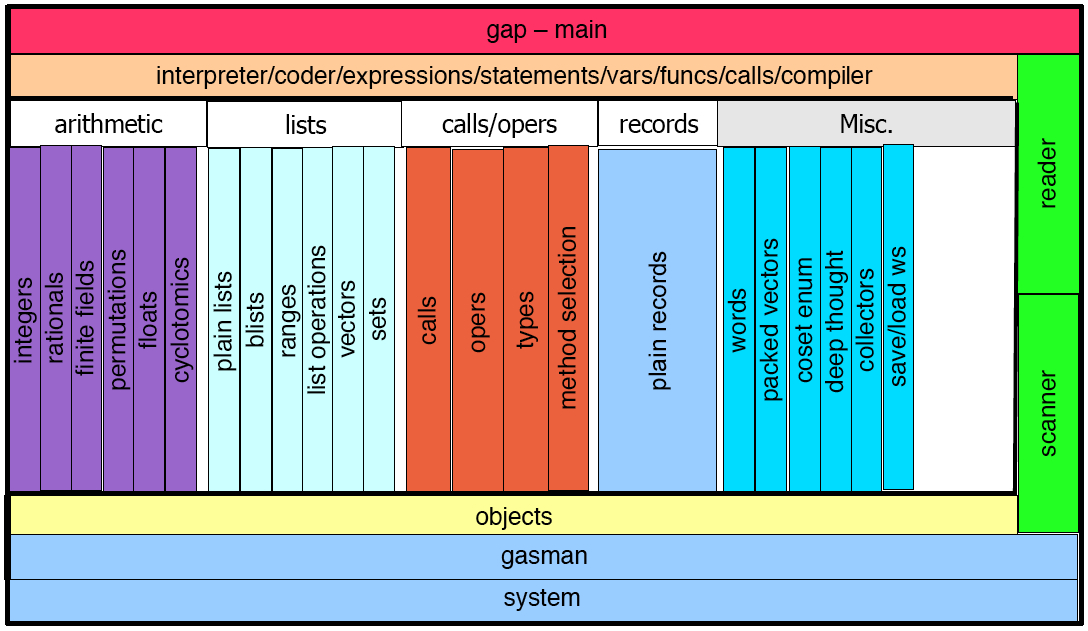
\includegraphics{bigpic.pdf}}}
   The 2nd line of the scheme, the
"interpreter/coder/expressions/statements/vars/funcs/calls/compiler" level is
essentially the \textsf{GAP} runtime system. It takes in \textsf{GAP} code and (possibly after parsing and storing it) executes it by calling
functions from the modules below. The GAP compiler is (a sort of) a drop in
replacement for this, and there could be others, such as a bytecode
generator/interpreter. 

 In the region within the thick lines the kernel code sees the same world as \textsf{GAP} code: it sees objects (including functions), with automatic management of
memory occupied by them. The only difference is that the kernel code can look,
if necessary, inside the binary content of the objects. 

 Unevaluated expressions or fragments of the \textsf{GAP} code never appear in this region and below it. Therefore, there are only a few
ways to pass control back from that level: 
\begin{itemize}
\item Calling a \textsf{GAP} function;
\item Entering a break loop;
\item Reading a file.
\end{itemize}
 }

 
\section{\textcolor{Chapter }{Garbage collection in \textsf{GAP}}}\label{Sect-Gasman}
\logpage{[ 2, 4, 0 ]}
\hyperdef{L}{X86BA4BA17AA4F56C}{}
{
  
\subsection{\textcolor{Chapter }{\textsf{GASMAN}}}\label{Subsect-Gasman}
\logpage{[ 2, 4, 1 ]}
\hyperdef{L}{X86E038D8796AECA3}{}
{
  \textsf{GASMAN} is the \textsf{GAP} memory manager. It provides an API dealing with \emph{Bags} which are areas of memory, each with a size and a \texttt{TNUM} (type number) in the range 0\texttt{\symbol{45}}\texttt{\symbol{45}}253 (type
numbers are defined in the file \texttt{objects.h}; there are some spare numbers reserved for further extensions; types 254 and
255 are reserved for \textsf{GASMAN}. See Section \ref{Sect-Objects} for more details). 

 Bags have stable handles (of \textsf{C} type \texttt{Bag}) and can be resized. When the heap is full, inaccessible bags are
automatically reclaimed and live bags may be moved, but the handles don't
change (handle is a pointer to a pointer to the actual data). Bag references
from \textsf{C} local variables are found automatically, and references from \textsf{C} static and global variables must be declared. \textsf{GASMAN} recovers unreachable bags automatically
\texttt{\symbol{45}}\texttt{\symbol{45}} it knows that bags in \textsf{C} local variables \emph{are} reachable. From the point of GC technicalities, \textsf{GASMAN} is generational, conservative, compacting (i.e. bags may move, but each has a
permanent ID) and cooperative (i.e. it imposes certain rules on its users)
memory manager. 

 To get the type of the bag with the identifier \texttt{b}, call \texttt{TNUM{\textunderscore}BAG(b)}. 

 The application specifies the type of a bag when it allocates it with \texttt{NewBag} and may later change it with \texttt{RetypeBag} (see \texttt{NewBag} and \texttt{RetypeBag} in \texttt{gasman.h}). 

 \textsf{GASMAN} needs to know the type of a bag so that it knows which function to call to
mark all subbags of a given bag (see \texttt{InitMarkFuncBags} below). Apart from that \textsf{GASMAN} does not care at all about types. }

 
\subsection{\textcolor{Chapter }{\textsf{GASMAN} Interface}}\label{Subsect-Gasman-Interface}
\logpage{[ 2, 4, 2 ]}
\hyperdef{L}{X7AA6E6517ED276FA}{}
{
  \texttt{Bag} is a type definition of some sort of pointer. It may be used as 
\begin{Verbatim}[commandchars=!@|,fontsize=\small,frame=single,label=]
  
  Bag bag = NewBag(type, size);
  
\end{Verbatim}
 Creation of a new bag may cause garbage collection, and \textsf{GAP} will fail if space cannot be allocated. 

 To reach the data in a bag, call 
\begin{Verbatim}[commandchars=!@|,fontsize=\small,frame=single,label=]
  
  Bag *ptr = PTR_BAG(bag);
  
\end{Verbatim}
 and keep in mind that the cost of such call is one indirection. 

 The \emph{key rule} is that you must NOT hold onto this pointer during any event which might cause
a garbage collection. A common hidden trap is to use 
\begin{Verbatim}[commandchars=!@|,fontsize=\small,frame=single,label=]
  
  PTR_BAG(list)[1] = NewBag(t,s);
  
\end{Verbatim}
 because the pointer may be evaluated before the right\texttt{\symbol{45}}hand
side evaluation, and used after it. Instead of this, you should use 
\begin{Verbatim}[commandchars=!@|,fontsize=\small,frame=single,label=]
  
  {
    Obj temp = NewBag(t,s);
    PTR_BAG(list)[1] = temp;
  }
  
\end{Verbatim}
 There is a second rule: after you assigned a bag identifier \texttt{b} into a bag \texttt{c} and before the next garbage collection, you must call \texttt{CHANGED{\textunderscore}BAG(c)}, unless you know that \texttt{b} cannot be garbage collected (e.g. it is an object like \texttt{true}), or \texttt{c} is the most recently allocated bag of all. 

 Other functions are: 
\begin{itemize}
\item  \texttt{RetypeBag( bag, newtnum )} changes the type of the bag with identifier \texttt{bag} to the new type \texttt{newtnum}. The identifier, the size, and also the address of the data area of the bag
do not change. 
\item  \texttt{ResizeBag( bag, newsize )} changes the size of the bag with identifier \texttt{bag} to the new size \texttt{newsize}. The identifier of the bag does not change, but the address of the data area
of the bag may change. If the new size is less than the old size, \textsf{GASMAN} throws away any data in the bag beyond the new size. If the new size is larger
than the old size, it extends the bag. Note that \texttt{ResizeBag} will perform a garbage collection if no free storage is available. During the
garbage collection the addresses of the data areas of all bags may change. So
you must not keep any pointers to or into the data areas of bags over calls to \texttt{ResizeBag} (see \texttt{PTR{\textunderscore}BAG} in \texttt{gasman.h}). 
\item  \texttt{InitMarkFuncBags( type, mark\texttt{\symbol{45}}func )}(optional) installs the function \texttt{mark\texttt{\symbol{45}}func} as marking function for bags of type \texttt{type}. The application \emph{must} install a marking function for a type before it allocates any bag of that
type. 

 A marking function returns nothing. It just takes a single argument of type \texttt{Bag} and applies the function \texttt{MarkBag} to each bag identifier that appears in the bag. During garbage collection
marking functions are applied to each marked bag (i.e. to all bags that are
assumed to be still live), to also mark their subbags. The ability to use the
correct marking function is the only use that \textsf{GASMAN} has for types. 

 \texttt{MarkBag(b)} marks the bag \texttt{b} as live so that it is not thrown away during a garbage collection. It tests if \texttt{bag} is a valid identifier of a bag in the young bags area. If it is not, then \texttt{MarkBag} does nothing, so there is no harm in calling it for something that is not
actually a bag identifier. It is important that \texttt{MarkBag} should only be called from the marking functions installed with \texttt{InitMarkFuncBags}. 

 \texttt{MarkBagWeakly} is an alternative to \texttt{MarkBag}, intended to be used by the marking functions of weak pointer objects. A bag
which is marked both weakly and strongly is treated as strongly marked. A bag
which is only weakly marked will be recovered by garbage collection, but its
identifier remains, marked in a way which can be detected by \texttt{IsWeakDeadBag}. This should always be checked before copying or using such an identifier. 

 \textsf{GASMAN} already provides the following standard marking functions defined in \texttt{gasman.c}: 
\begin{itemize}
\item  \texttt{MarkNoSubBags( bag )} is a marking function for types whose bags contain no identifier of other
bags. It does nothing, as its name implies, and simply returns. For example,
the bags for large integers contain only the digits and no identifiers of
bags. 
\item  \texttt{MarkOneSubBags( bag )} is a marking function for types whose bags contain exactly one identifier of
another bag as the first entry. It marks this subbag and returns. For example,
bags for finite field elements contain exactly one bag identifier for the
finite field the element belongs to. 
\item  \texttt{MarkTwoSubBags( bag )} is a marking function for types whose bags contain exactly two identifiers of
other bags as the first and second entry such as the binary operations bags.
It marks those subbags and returns. For example, bags for rational numbers
contain exactly two bag identifiers for the numerator and the denominator. 
\item  \texttt{MarkAllSubBags( bag )} is the marking function for types whose bags contain only identifiers of other
bags (for example, bags or lists contain only bag identifiers for the elements
of the list or 0 if an entry has no assigned value). \texttt{MarkAllSubBags} marks every entry of such a bag. Note that \texttt{MarkAllSubBags} assumes that all identifiers are at offsets from the address of the data area
of \texttt{bag} that are divisible by \texttt{sizeof(Bag)}. Also, since it does not do any harm to mark something which is not actually
a bag identifier, one could use \texttt{MarkAllSubBags} for all types as long as the identifiers in the data area are properly aligned
as explained above (this would however slow down \texttt{CollectBags}). By default, \textsf{GASMAN} uses \texttt{MarkAllSubBagsDefault} which does exactly this. 
\end{itemize}
 
\end{itemize}
 }

 
\subsection{\textcolor{Chapter }{The GASMAN Interface for Weak Pointer Objects}}\label{The GASMAN Interface for Weak Pointer Objects}
\logpage{[ 2, 4, 3 ]}
\hyperdef{L}{X7C1EFEEB8071E0A2}{}
{
  The key support for weak pointers is in the files \texttt{src/gasman.c} and \texttt{src/gasman.h}. This document assumes familiarity with the rest of the operation of GASMAN.
A kernel type (tnum) of bags which are intended to act as weak pointers to
their subobjects must meet three conditions. Firstly, the marking function
installed for that tnum must use \texttt{MarkBagWeakly} for those subbags, rather than \texttt{MarkBag}. Secondly, before any access to such a subbag, it must be checked with \texttt{IsWeakDeadBag}. If that returns \texttt{true}, then the subbag has evaporated in a recent garbage collection and must not
be accessed. Typically the reference to it should be removed. Thirdly, a \emph{sweeping function} must be installed for that tnum which copies the bag, removing all references
to dead weakly held subbags. 

 The files \texttt{src/weakptr.c} and \texttt{src/weakptr.h} use this interface to support weak pointer objects. Other objects with weak
behaviour could be implemented in a similar way. }

 }

 
\section{\textcolor{Chapter }{Interfaces}}\label{Sect-Interfaces}
\logpage{[ 2, 5, 0 ]}
\hyperdef{L}{X815C2D007A090300}{}
{
  The modules at the bottom of the picture from the section \ref{Sect-BigPicture} (\emph{objects}, \emph{gasman} and \emph{system}), and white boxes (\emph{arithmetic}, \emph{lists}, \emph{calls/operations}, \emph{records}) provide interfaces intended for use in the kernel. 

 For example \texttt{ariths.h} provides functions like \texttt{SUM}, \texttt{PROD}, \texttt{AINV}, corresponding to the GAP operations \texttt{+}, \texttt{*} and unary \texttt{\texttt{\symbol{45}}}. These functions can be applied to any values (objects) to perform an
appropriate action. Note that there is some overhead in using these general
functions, if you know what your arguments are, there may be faster ways. 

 Another interface provides \texttt{ELM{\textunderscore}LIST}, \texttt{ASS{\textunderscore}LIST}, \texttt{LEN{\textunderscore}LIST}, etc. as a general interface to any type of list. 

 Functions like these will even work for \textsf{GAP}\texttt{\symbol{45}}level objects whose arithmetic or list operations are
implemented by installed methods. 

 Adding a kernel function is easy if it stays in the region within the thick
lines, i.e. it uses interfaces from white and yellow areas, which provide
kernel equivalents to the basic GAP functionality. 

 For example, the following kernel function will return a list containing an
object, its square and its cube: 
\begin{Verbatim}[commandchars=!@|,fontsize=\small,frame=single,label=Example]
  
  /*  x -> [x,x^2,x^3]  */
  static Obj FuncFoo1(Obj self, Obj x)
  {
      Obj x2, x3;
      Obj list = NEW_PLIST( T_PLIST, 3 );
      SET_ELM_PLIST( list, 1, x );
      CHANGED_BAG( list );
  
      x2 = PROD( x, x );
      SET_ELM_PLIST( list, 2, x2 );
      CHANGED_BAG( list );
  
      x3 = PROD( x2, x );
      SET_ELM_PLIST( list, 3, x3 );
      CHANGED_BAG( list );
  
      SET_LEN_PLIST(list, 3);
      return list;
  }
  
\end{Verbatim}
 If speed is not of utmost importance, then it is usually better to use the \texttt{ASS{\textunderscore}LIST} etc. functions instead of \texttt{SET{\textunderscore}ELM{\textunderscore}PLIST} and friends, which are more low\texttt{\symbol{45}}level and easier to misuse.
For example, they automatically call \texttt{CHANGED{\textunderscore}BAG} and \texttt{SET{\textunderscore}LEN{\textunderscore}PLIST}. Then the above example would become this instead: 
\begin{Verbatim}[commandchars=!@|,fontsize=\small,frame=single,label=Example]
  
  /*  x -> [x,x^2,x^3]  */
  static Obj FuncFoo2(Obj self, Obj x)
  {
      Obj x2, x3;
      Obj list = NEW_PLIST( T_PLIST, 3 );
      ASS_LIST( list, 1, x );
  
      x2 = PROD( x, x );
      ASS_LIST( list, 2, x2 );
  
      x3 = PROD( x2, x );
      ASS_LIST( list, 3, x3 );
  
      return list;
  }
  
\end{Verbatim}
 Finally, if all you want to do is produce a list of fixed length, you can use
the \texttt{NewPlistFromArgs} helper function: 
\begin{Verbatim}[commandchars=!@|,fontsize=\small,frame=single,label=Example]
  
  /*  x -> [x,x^2,x^3]  */
  Obj FuncFoo3(Obj self, Obj x)
  {
      Obj x2 = PROD( x, x );
      Obj x3 = PROD( x2, x );
      return NewPlistFromArgs( x, x2, x3 );
  }
  
\end{Verbatim}
 }

 
\section{\textcolor{Chapter }{Objects and API}}\label{Sect-Objects}
\logpage{[ 2, 6, 0 ]}
\hyperdef{L}{X849901607E91AC92}{}
{
  The kernel representation of every \textsf{GAP} object is an object of \textsf{C} type \texttt{Obj}. Objects are defined in the file \texttt{objects.h}. Objects are actually \emph{bags} (represented by their handles), small integers and small finite field elements
(represented by values that could not be valid handles). \texttt{Bag} is the type of bag identifiers, defined in the file \texttt{system.h}: 
\begin{Verbatim}[commandchars=!@|,fontsize=\small,frame=single,label=Example]
  
  typedef UInt * *        Bag;
  
\end{Verbatim}
 Each bag is identified by its \emph{bag identifier}, and no two live bags have the same identifier. 

 Note that the identifier of a bag is different from the address of the data
area of the bag. This address may change during a garbage collection while the
identifier of a bag never changes. Bags that contain references to other bags
must always contain the identifiers of these other bags, never the addresses
of the data areas of the bags. 

 Note that bag identifiers are recycled. That means that after a bag dies its
identifier may be reused for a new bag. 

 0 is a valid value of the type \texttt{Bag}, but is guaranteed not to be the identifier of any bag. 

 The ability to distinguish between bags and other objects relies on the fact
that all bag identifiers are divisible by 4. 

 There are lots of kernel API functions providing a uniform interface for
working with objects: 
\begin{itemize}
\item  \texttt{TNUM{\textunderscore}OBJ} (first level type), \texttt{SIZE{\textunderscore}OBJ}, \texttt{ADDR{\textunderscore}OBJ} (C pointer to data), \texttt{TYPE{\textunderscore}OBJ} (full type) 
\item  \texttt{IS{\textunderscore}MUTABLE{\textunderscore}OBJ}, \texttt{MakeImmutable}, \texttt{COPY{\textunderscore}OBJ}, ... 
\item  \texttt{PRINT{\textunderscore}OBJ} 
\item  \texttt{NEW{\textunderscore}PLIST}, \texttt{SET{\textunderscore}ELM{\textunderscore}PLIST}, etc. for creating plain lists 
\item  \texttt{PROD} for arithmetic (see also \texttt{SUM}, \texttt{DIFF}, etc.) 
\end{itemize}
 These functions are flexible: for example, \texttt{PROD} will multiply anything, but if you know what objects you will have it will be
a bit faster to call the multiplication directly. 

 Typical implementation is a table of functions indexed by \texttt{TNUM{\textunderscore}OBJ}. For example, this is the definition of \texttt{PROD} in the file \texttt{ariths.h} (you can safely ignore the \texttt{EXPORT{\textunderscore}INLINE} for now): 
\begin{Verbatim}[commandchars=!@|,fontsize=\small,frame=single,label=Example]
  
  EXPORT_INLINE Obj PROD(Obj opL, Obj opR)
  {
      UInt tnumL = TNUM_OBJ(opL);
      UInt tnumR = TNUM_OBJ(opR);
      return (*ProdFuncs[tnumL][tnumR])(opL, opR);
  }
  
\end{Verbatim}
 Additionally, \texttt{objects.h} also defines symbolic names for TNUMs. 

 There are lots of other API functions for strings, general lists, calling
functions, etc. 
\subsection{\textcolor{Chapter }{Immediate Integers and FFEs}}\label{Subsect-Integers}
\logpage{[ 2, 6, 1 ]}
\hyperdef{L}{X7B314E837FD109B1}{}
{
  There are three integer types in GAP: \texttt{T{\textunderscore}INT}, \texttt{T{\textunderscore}INTPOS} and \texttt{T{\textunderscore}INTNEG}. Each integer has a unique representation, e.g., an integer that can be
represented as \texttt{T{\textunderscore}INT} is never represented as \texttt{T{\textunderscore}INTPOS} or \texttt{T{\textunderscore}INTNEG}. 

 \texttt{T{\textunderscore}INT} is the type of those integers small enough to fit into 29 bits (on 32 bit
systems) respectively 61 bits (on 64 bit systems). Therefore the value range
of this small integers is $-2^{28}...2^{28}-1$ respectively $-2^{60}...2^{60}-1$. Only these small integers can be used as index expression into sequences. 

 Small integers are represented by an immediate integer handle, containing the
value instead of pointing to it, which has the format \texttt{ss{\textless}28 data bits{\textgreater}01} respectively \texttt{ss{\textless}60 data bits{\textgreater}01}. 

 Immediate integers handles carry the tag \texttt{T{\textunderscore}INT}, i.e. the last bit is 1. Thus, the last bit distinguishes immediate integers
from other handles which point to structures aligned on 4 byte (on 32 bit)
respectively 8 byte (on 64 bit) boundaries and therefore have last bit zero.
(The bit before the last is reserved as tag to allow extensions of this
scheme.) Using immediates as pointers and dereferencing them gives address
errors. 

 The first two bits \texttt{ss} are two copies of the sign bit. That is, the sign bit of immediate integers
has a guard bit, that allows quick detection of overflow for addition since
these two bits must always be equal. 

 Functions \texttt{IS{\textunderscore}INTOBJ} and \texttt{ARE{\textunderscore}INTOBJS} are used to test if an object (or two objects) is an (immediate) integer
object. The functions \texttt{INTOBJ{\textunderscore}INT} is used to convert a \textsf{C} integer to an (immediate) integer object, and \texttt{INT{\textunderscore}INTOBJ} is used to convert the (immediate) integer object to a \textsf{C} integer. These functions do NOT check for overflows. 

 The other two integer types are \texttt{T{\textunderscore}INTPOS} and \texttt{T{\textunderscore}INTNEG} for positive (respectively, negative) integer values that cannot be
represented by immediate integers. See comments in \texttt{integer.c} for details. 

 Other immediate objects are \emph{finite field elements} (FFEs). The kernel supports small finite fields with up to 65536 elements
(larger fields can be realized as polynomial domains over smaller fields).
Immediate FFEs are represented in the format \texttt{{\textless}16 bit value{\textgreater}{\textless}13 bit field
ID{\textgreater}010}, where the least significant 3 bits of such an immediate object are always
010, flagging the object as an object of a small finite field. 

 The next 13 bits represent the small finite field where the element lies, and
they are simply an index into a global table of small finite fields. 

 The most significant 16 bits represent the value of the element. 

 If the value is 0, then the element is the zero from the finite field.
Otherwise the integer is the logarithm of this element with respect to a fixed
generator of the multiplicative group of the finite field plus one. In the
following descriptions we denote this generator always with $z$, it is an element of order $ord-1$, where $ord$ is the order of the finite field. Thus 1 corresponds to $z^{1-1} = z^0 = 1$, i.e., the one from the field. Likewise 2 corresponds to $z^{2-1} = z^1 = z$, i.e., the root itself. 

 This representation makes multiplication very easy, we only have to add the
values and subtract 1 , because $z^{a-1} * z^{b-1} = z^{(a+b-1)-1}$. Addition is reduced to multiplication by the formula $z^a + z^b = z^b * (z^{a-b}+1)$. This makes it necessary to know the successor $z^a + 1$ of every value. 

 The finite field bag contains the successor for every nonzero value, i.e., \texttt{SUCC{\textunderscore}FF({\textless}ff{\textgreater})[{\textless}a{\textgreater}]} is the successor of the element \texttt{{\textless}a{\textgreater}}, i.e, it is the logarithm of $z^{a-1} + 1$. This list is usually called the Zech\texttt{\symbol{45}}Logarithm table. The
zeroth entry in the finite field bag is the order of the finite field minus
one. 

 \texttt{T{\textunderscore}INT} and \texttt{T{\textunderscore}FFE} are reserved \texttt{TNUM}s for immediate integers and FFEs. \texttt{TNUM{\textunderscore}OBJ} produces them if needed and otherwise calls \texttt{TNUM{\textunderscore}BAG}. 

 The kernel design allows that other immediate types could be added in the
future. }

 
\subsection{\textcolor{Chapter }{Arithmetics}}\label{Subsect-Arithmetics}
\logpage{[ 2, 6, 2 ]}
\hyperdef{L}{X87FF26F4878230FB}{}
{
  Arithmetic operations package is implemented in files \texttt{ariths.h} and \texttt{ariths.c}. In particular, it defines functions like \texttt{SUM(obj1, obj2)}, \texttt{DIFF}, \texttt{PROD} etc., which accept (and may return) objects of any kind, including immediate
objects. Selection of the appropriate method is handled via calling \texttt{TNUM{\textunderscore}OBJ} for arguments and then calling the appropriate method from the table of
functions, for example: 
\begin{Verbatim}[commandchars=!@|,fontsize=\small,frame=single,label=]
  
  EXPORT_INLINE Obj SUM(Obj opL, Obj opR)
  {
      UInt tnumL = TNUM_OBJ(opL);
      UInt tnumR = TNUM_OBJ(opR);
      return (*SumFuncs[tnumL][tnumR])(opL, opR);
  }
  
\end{Verbatim}
 The default entry of the table of functions just calls back to the \textsf{GAP} level to look for the installed methods (see e.g. \texttt{SumObject} in \texttt{ariths.c}), but note that kernel methods installed in tables \emph{OVERRIDE} \textsf{GAP} installed methods. 

 If you expect to handle mainly small integers, then it is significantly faster
to do: 
\begin{Verbatim}[commandchars=@CD,fontsize=\small,frame=single,label=]
  
  if ( ! ARE_INTOBJS( <opL>, <opR> ) || ! SUM_INTOBJS( <res>, <opL>, <opR> ) )
      <res> = SUM( <opL>, <opR> );
  
\end{Verbatim}
 instead of \texttt{{\textless}res{\textgreater} = SUM({\textless}opL{\textgreater},
{\textless}opR{\textgreater})}, where \texttt{SUM{\textunderscore}INTOBJS} is a function, which returns 0 if the answer overflows and a large integer
needs to be created. 

 Finally, note that lots of functions in \texttt{ariths.h} called \texttt{C{\textunderscore}{\textless}something{\textgreater}} are used mainly by the compiler. }

 
\subsection{\textcolor{Chapter }{Functions}}\label{Subsect-Functions}
\logpage{[ 2, 6, 3 ]}
\hyperdef{L}{X86FA580F8055B274}{}
{
  The function call mechanism package is implemented in files \texttt{calls.h} and \texttt{calls.c}. A function object in \textsf{GAP} is represented by a bag of the type \texttt{T{\textunderscore}FUNCTION}. The bag for the function \texttt{f} contains eight pointers fo \textsf{C} functions \texttt{\symbol{45}} its handlers. These eight functions are for
0,1,2,...,6 arguments and X arguments respectively, and the $i$\texttt{\symbol{45}}th handler can be accessed using the function \texttt{HDLR{\textunderscore}FUNC(f, i)}. This is exactly what is done by functions \texttt{CALL{\textunderscore}0ARGS}, \texttt{CALL{\textunderscore}1ARGS}, ..., \texttt{CALL{\textunderscore}6ARGS} and \texttt{CALL{\textunderscore}XARGS}, which simply call the appropriate handlers, passing the function bag and the
arguments. \texttt{CALL{\textunderscore}0ARGS} is for calls passing no arguments, \texttt{CALL{\textunderscore}1ARGS} is for calls passing one argument, and so on. Thus, the kernel equivalent of
the GAP code \texttt{r := f(a,b)} is \texttt{r = CALL{\textunderscore}2ARGS(f,a,b)}. \texttt{CALL{\textunderscore}XARGS} is for calls passing more than 6 arguments or for variadic functions, and it
requires the arguments to be collected in a single plain list. 

 There is a range of standard handlers that deal with calls to regular \textsf{GAP} functions, to operations, attributes and properties and that also deal with \textsf{GAP} variadic functions given as \texttt{function(arg)}. 

 For kernel functions, the handler is the actual function which does the work.
A typical handler (for 1\texttt{\symbol{45}}argument function) looks like 
\begin{Verbatim}[commandchars=!@|,fontsize=\small,frame=single,label=]
  
  Obj FuncLength(Obj self, Obj list)
  {
      return INTOBJ_INT(LEN_LIST(list));
  }
  
\end{Verbatim}
 Often the handler has to do some checks on arguments as well. In the example
above \texttt{LEN{\textunderscore}LIST} takes care of this (mainly because the jump table for \texttt{LEN{\textunderscore}LIST} contains error functions for non\texttt{\symbol{45}}lists). Every handler must
be registered (once) with a unique ``cookie'' by calling \texttt{InitHandlerFunc( handler, cookie )} before it is installed in any function bag. This is needed so that it can be
identified when loading a saved workspace. \mbox{\texttt{\mdseries\slshape cookie}} should be a unique \textsf{C} string, identifying the handler. 

 To create a function object, there are three functions \texttt{NewFunction}, \texttt{NewFunctionC}, and \texttt{NewFunctionT}, defined in the file \texttt{calls.c}. 

 \texttt{NewFunction( name, narg, nams, hdlr )} creates and returns a new function. \mbox{\texttt{\mdseries\slshape name}} must be a \textsf{GAP} string containing the name of the function. \mbox{\texttt{\mdseries\slshape narg}} must be the number of arguments, where \texttt{\symbol{45}}1 indicates a
variable number of arguments. \mbox{\texttt{\mdseries\slshape nams}} must be a \textsf{GAP} list containing the names of the arguments. \mbox{\texttt{\mdseries\slshape hdlr}} must be the \textsf{C} function (accepting \mbox{\texttt{\mdseries\slshape self}} and the \mbox{\texttt{\mdseries\slshape narg}} arguments) that will be called to execute the function. 

 \texttt{NewFunctionC} does the same as \texttt{NewFunction}, but expects \mbox{\texttt{\mdseries\slshape name}} and \mbox{\texttt{\mdseries\slshape nams}} as \textsf{C} strings. \texttt{NewFunctionT} also does the same as \texttt{NewFunction}, but has two extra arguments that allow to specify the \mbox{\texttt{\mdseries\slshape type}} and \mbox{\texttt{\mdseries\slshape size}} of the newly created bag. 

 For example, you can make a function object using the code like this: 
\begin{Verbatim}[commandchars=!@|,fontsize=\small,frame=single,label=]
  
  lenfunc = NewFunctionC("Length", 1, "list", FuncLength);
  
\end{Verbatim}
 }

 
\subsection{\textcolor{Chapter }{Lists}}\label{Subsect-Lists}
\logpage{[ 2, 6, 4 ]}
\hyperdef{L}{X7B256AE5780F140A}{}
{
  The \textsf{GAP} kernel provides a generic list interface, which is equivalent to using \texttt{list[i]} etc. in the library. This interface works for all types of lists known to GAP,
including virtual lists. It has functions like \texttt{IS{\textunderscore}LIST} (returns \textsf{C} Boolean), \texttt{LEN{\textunderscore}LIST} (returns \textsf{C} integer), \texttt{ISB{\textunderscore}LIST}, \texttt{ELM{\textunderscore}LIST}, \texttt{ELM0{\textunderscore}LIST( {\textless}list{\textgreater},
{\textless}pos{\textgreater} ) } (returns 0 if {\textless}list{\textgreater} has no assigned object at position
{\textless}pos{\textgreater}) and \texttt{ASS{\textunderscore}LIST}, defined in the file \texttt{lists.h} Implementation of these functions is done via tables of functions indexed by
TNUM. 

 Nevertheless, it will be not much faster to write your \textsf{C} code using such functions, for example, to reverse an arbitrary list, than to
do the same working in \textsf{GAP}. However, in case of \emph{plain lists} coding in \textsf{C} actually ought to produce some speedup. 

 A plain list is a list that may have holes and may contain elements of
arbitrary types. A plain list may also have room for elements beyond its
current logical length. The last position to which an element can be assigned
without resizing the plain list is called the physical length. 

 If you need to create a plain list, use \texttt{NEW{\textunderscore}PLIST({\textless}tnum{\textgreater},{\textless}plength{\textgreater})}, where \texttt{{\textless}tnum{\textgreater}} should be \texttt{T{\textunderscore}PLIST{\textunderscore}{\textless}something{\textgreater}}, and \texttt{{\textless}plength{\textgreater}} is physical length in bags. Furthermore, \texttt{LEN{\textunderscore}PLIST} gets its logical length, and \texttt{SET{\textunderscore}LEN{\textunderscore}PLIST} sets its logical length. Note that \texttt{ELM{\textunderscore}PLIST} is faster than \texttt{ELM{\textunderscore}LIST}. }

 
\subsection{\textcolor{Chapter }{Data objects}}\label{Subsect-Data-Objects}
\logpage{[ 2, 6, 5 ]}
\hyperdef{L}{X789D77787E3527D4}{}
{
  \emph{Positional} and \emph{Component} objects are made from lists and records using \texttt{Objectify}. They contain their \emph{Type} and data accessible with \texttt{![]} and \texttt{!.} operations. 

 \emph{Data objects} also contain their \emph{Type}, but the data is only accessible via kernel functions. Data can be anything
you like \emph{except} bag references. The garbage collector doesn't see inside them. At a minimum,
construction and basic access functions need to be written in the kernel. For
example, compressed vectors are done this way. }

 }

 
\section{\textcolor{Chapter }{Rules of Kernel Programming}}\label{Sect-Rules}
\logpage{[ 2, 7, 0 ]}
\hyperdef{L}{X7A547AB487DA5FA9}{}
{
  
\subsection{\textcolor{Chapter }{Three golden rules}}\label{Sect-GoldenRules}
\logpage{[ 2, 7, 1 ]}
\hyperdef{L}{X861B9EB587F6B238}{}
{
  Three golden rules of \textsf{GAP} kernel programming: 
\begin{enumerate}
\item  Real \textsf{C} pointers into objects (returned by \texttt{ADDR{\textunderscore}OBJ}) must \emph{not} be held across anything that could cause a garbage collection (\emph{GC}). 
\item  If you add a new object to another one (e.g. put it in a list) you must call \texttt{CHANGED{\textunderscore}BAG} on the container, otherwise the new object may get lost in a GC. 
\item  Don't use malloc: actually using it a little bit is usually safe, and it's
safe if you don't ever want to expand the GAP workspace. 
\end{enumerate}
 }

 
\subsection{\textcolor{Chapter }{Common kernel traps}}\label{Subsect-Traps}
\logpage{[ 2, 7, 2 ]}
\hyperdef{L}{X8055D4158291EAA2}{}
{
  More things can cause a garbage collection than you expect: 
\begin{itemize}
\item printing (might be to string stream)
\item generic list or record access (might be handled by \textsf{GAP} methods)
\item integer arithmetic (might overflow to large integers)
\end{itemize}
 Be careful of things like 
\begin{Verbatim}[commandchars=!@|,fontsize=\small,frame=single,label=Example]
  
  ELM_PLIST(l, 3) = something that might cause GC
  
\end{Verbatim}
 This expands in \textsf{C} to \texttt{*((*l)+3) = something}. The compiler is allowed to follow the inner *, then evaluate the
right\texttt{\symbol{45}}hand side, then the outer *. This will be broken by
the garbage collection. }

 
\subsection{\textcolor{Chapter }{One More Bit of GASMAN interface}}\label{Subsect-MoreGasman}
\logpage{[ 2, 7, 3 ]}
\hyperdef{L}{X7FC1A0FA7B0E8554}{}
{
  When you store a Bag ID in a \textsf{C} global variable, you must declare the address of the global to \textsf{GASMAN} (so the GC knows that the bag is alive). This is done by calling \texttt{InitGlobalBag} passing the address and another "cookie" which is used by save/load. 

 There are nice ways to do all the global and handler initializations from
tables. }

 }

 
\section{\textcolor{Chapter }{The \textsf{GAP} compiler}}\label{Sect-compiler}
\logpage{[ 2, 8, 0 ]}
\hyperdef{L}{X82DBFB18873C8E8F}{}
{
  
\subsection{\textcolor{Chapter }{Compiling \textsf{GAP} Code}}\label{Compiling GAP Code}
\logpage{[ 2, 8, 1 ]}
\hyperdef{L}{X7AFA67497FA81DCD}{}
{
  The \textsf{GAP} compiler converts \textsf{GAP} code into kernel functions. The compiled code then can be loaded into a
running kernel (on UNIX or Mac OS). The resulting code still has to do lots of
checks, so usually it will not be as fast as hand\texttt{\symbol{45}}written \textsf{C} program. The performance gain is significant for code that spends a lot of
time in loops, small integer arithmetic, etc., and will be not significant if
code spends most of its time in the kernel or elsewhere in library. 

 In the following example we compile the file \texttt{foo.g} and then load it during the subsequent \textsf{GAP} session: 
\begin{Verbatim}[commandchars=!@|,fontsize=\small,frame=single,label=Example]
  
  $ cat > foo.g
  foo := x -> [x,x^2,x^3];
  $ gac -d -C foo.g
  ... compilation to C file ...
  $ gac -d foo.g
  ... compilation to .so file ...
  $ ls -l foo.so
  -rwxr-xr-x 1 sal 158 4999 2007-09-11 10:19 foo.so*
  $ gap -b
  GAP4, Version: 4.dev of today, ....
  !gapprompt@gap>| !gapinput@LoadDynamicModule("./foo.so");|
  !gapprompt@gap>| !gapinput@Print(foo);|
  function ( x )
      <<compiled GAP code>> from foo.g:1
  end
  !gapprompt@gap>| !gapinput@foo(3);|
  [ 3, 9, 27 ]
  
\end{Verbatim}
 The compiler code will look as follows: 
\begin{Verbatim}[commandchars=!@|,fontsize=\small,frame=single,label=Example]
  
  /* return [ x, x ^ 2, x ^ 3 ]; */
  t_1 = NEW_PLIST( T_PLIST, 3 );
  SET_LEN_PLIST( t_1, 3 );
  SET_ELM_PLIST( t_1, 1, a_x );
  CHANGED_BAG( t_1 );
  t_2 = POW( a_x, INTOBJ_INT(2) );
  SET_ELM_PLIST( t_1, 2, t_2 );
  CHANGED_BAG( t_1 );
  t_2 = POW( a_x, INTOBJ_INT(3) );
  SET_ELM_PLIST( t_1, 3, t_2 );
  CHANGED_BAG( t_1 );
  SWITCH_TO_OLD_FRAME(oldFrame);
  return t_1;
  
\end{Verbatim}
 Note that the original \textsf{GAP} code (more or less) appears as comments. 

 If you want to see or modify the intermediate \textsf{C} code, you can also instruct the compiler to produce only the \textsf{C} files by using the option \texttt{\texttt{\symbol{45}}C} instead of \texttt{\texttt{\symbol{45}}d}. 

 There are some known problems with \textsf{C} code produced with the \textsf{GAP} compiler on 32 bit architectures and used on 64 bit architectures (and vice
versa). 

 There are more ways to exploit the \textsf{GAP} compiler apart from just compiling the \textsf{GAP} code: 
\begin{itemize}
\item You can compile your code and then hand\texttt{\symbol{45}}optimize critical
sections. For example, you can replace calls to \texttt{POW} by calls to \texttt{PROD} or even to the product function for particular kinds of objects. You must be
aware of a risk of a segmentation fault if you will call your function with
wrong arguments. 
\item  You can use the compiler to generate a shell that can be dynamically loaded,
and then fill in your own \textsf{C} code in this shell. This approach is used in \textsf{Browse}, \textsf{EDIM} and \textsf{IO} packages. In this case you must make it sure that your code complies with
rules. 
\end{itemize}
 }

  
\subsection{\textcolor{Chapter }{Suitability for Compilation}}\label{Suitability for Compilation}
\logpage{[ 2, 8, 2 ]}
\hyperdef{L}{X7FBB45C17D3F3B0B}{}
{
  Typically algorithms spend large parts of their runtime only in small parts of
the code. The design of \textsf{GAP} reflects this situation with kernel methods for many time critical
calculations such as matrix or permutation arithmetic. 

 Compiling an algorithm whose time critical parts are already in the kernel of
course will give disappointing results: Compilation will only speed up the
parts that are not already in the kernel and if they make us a small part of
the runtime, the overall gain is small. 

 Routines that benefit from compilation are those which do extensive operations
with basic data types, such as lists or small integers. }

 }

 
\section{\textcolor{Chapter }{Global Variables}}\label{Sect-GVars}
\logpage{[ 2, 9, 0 ]}
\hyperdef{L}{X7D9044767BEB1523}{}
{
  
\subsection{\textcolor{Chapter }{Global variables}}\label{Subsect-GVars}
\logpage{[ 2, 9, 1 ]}
\hyperdef{L}{X7D9044767BEB1523}{}
{
  The part of the kernel that manages global variables, i.e., the global
namespace, is contained in the files \texttt{gvars.h} and \texttt{gvars.c}. Global variables have an internal form, of type \texttt{GVar} (actually an index into a hash table). They may be obtained with \texttt{GVar gv = GVarName({\textless}string{\textgreater});}. A global variable may be safely held on to across GC (but not across
save/load workspace). 

 To manipulate with global variables, you may use \texttt{AssGVar(gv, {\textless}obj{\textgreater})} or \texttt{ValGVar( gv )} (returns 0 if unbound, not an error), etc. }

 
\subsection{\textcolor{Chapter }{Tracking global variables}}\label{Subsect-TrackGVars }
\logpage{[ 2, 9, 2 ]}
\hyperdef{L}{X7A106F327F75851A}{}
{
  The \textsf{C} code 
\begin{Verbatim}[commandchars=!@|,fontsize=\small,frame=single,label=]
  
  Obj Stuff;
  InitCopyGVar( "stuff", &Stuff );
  
\end{Verbatim}
 causes \texttt{Stuff} to track the value of the global named "stuff". When the global is changed,
the new value will be put in the \textsf{C} variable. 

 A useful refinement is \texttt{InitFopyGVar}. This does the same, provided that the value assigned is a function,
otherwise the \textsf{C} variable points to a function that prints a suitable error message. 

 These are usually set up during initialization of a kernel module. }

 }

 
\section{\textcolor{Chapter }{The Kernel Module Structure and interface}}\label{Sect-Kernel-Modules}
\logpage{[ 2, 10, 0 ]}
\hyperdef{L}{X7B6775AC8609D5AB}{}
{
  
\subsection{\textcolor{Chapter }{The Kernel Module Structure}}\label{Subsect-Kernel-Modules-Structure}
\logpage{[ 2, 10, 1 ]}
\hyperdef{L}{X82E5407283B16176}{}
{
  Apart from a very small amount of glue, all of the kernel (including compiled
GAP code) is organised into modules. 

 Basically each module consists of one \texttt{.c} file and one \texttt{.h} file. The file \texttt{gap.c} contains the variable \texttt{InitFuncsBuiltinModules} which is initialized with a list of functions such as \texttt{InitInfoInt}. Each such function, when called, returns a data structure describing a
module, which typically looks as follows: 
\begin{Verbatim}[commandchars=!@|,fontsize=\small,frame=single,label=]
  
  /****************************************************************************
  **
  *F  InitInfoInt() . . . . . . . . . . . . . . . . . . table of init functions
  */
  static StructInitInfo module = {
      .type = MODULE_BUILTIN,
      .name = "integer",
      .initKernel = InitKernel,
      .initLibrary = InitLibrary,
  };
  
\end{Verbatim}
 The first part is just information, but the functions from \texttt{initKernel} down are the key to the interface to kernel modules. }

 
\subsection{\textcolor{Chapter }{The Kernel Module Interface}}\label{Subsect-Kernel-Modules-Interface}
\logpage{[ 2, 10, 2 ]}
\hyperdef{L}{X875A1DC186FEC3C5}{}
{
  The general rule is that if a 0 appears, the function is skipped; indeed, you
may omit entries which are 0.

 When GAP is starting up, it does the following: 
\begin{itemize}
\item Calls the \texttt{initKernel} functions of all those modules that have one. If any of them return
non\texttt{\symbol{45}}zero then it aborts.
\item Then calls the \texttt{initLibrary} functions likewise
\item Then the \texttt{checkInit} functions
\end{itemize}
 The other three functions relate to save/load workspace: 
\begin{itemize}
\item \texttt{preSave} functions are called before saving.
\item \texttt{postSave} functions (in the reverse order) after saving
\item \texttt{postRestore} functions are called after a workspace has been loaded to finish linking up
the kernel and workspace.
\end{itemize}
 }

 
\subsection{\textcolor{Chapter }{Sequences of Events}}\label{Subsect-SeqEvents}
\logpage{[ 2, 10, 3 ]}
\hyperdef{L}{X7FBC8CDB82C7A500}{}
{
  Normal GAP startup (no \texttt{\symbol{45}}L) 
\begin{itemize}
\item All \texttt{initKernel} methods called (abort on non\texttt{\symbol{45}}zero return)
\item All \texttt{initLibrary} methods called (abort on non\texttt{\symbol{45}}zero return)
\item All \texttt{checkInit} methods called (abort on non\texttt{\symbol{45}}zero return)
\item \texttt{init.g} read
\end{itemize}
 Startup loading a workspace 
\begin{itemize}
\item All \texttt{initKernel} methods called (abort on non\texttt{\symbol{45}}zero return)
\item Workspace loaded, global bags and handlers linked up
\item All \texttt{postRestore} methods called (abort on non\texttt{\symbol{45}}zero return)
\item Enter the main loop
\end{itemize}
 }

 
\subsection{\textcolor{Chapter }{Saving a Workspace}}\label{Subsect-Workspace}
\logpage{[ 2, 10, 4 ]}
\hyperdef{L}{X80CAC88A7E9561E3}{}
{
  
\begin{itemize}
\item All \texttt{preSave} methods called (recover on non\texttt{\symbol{45}}zero return)
\item Full garbage collection
\item After this, workspace must be "clean" \texttt{\symbol{45}}\texttt{\symbol{45}}
no non\texttt{\symbol{45}}objects stored where objects are expected (eg in
plain lists)
\item Saved workspace file written
\item All \texttt{postSave} methods called in reverse order
\end{itemize}
 }

 
\subsection{\textcolor{Chapter }{Excerpts from InitKernel from integer.c}}\label{Subsect-Excerpts}
\logpage{[ 2, 10, 5 ]}
\hyperdef{L}{X809F94777E699351}{}
{
  
\begin{Verbatim}[commandchars=!@|,fontsize=\small,frame=single,label=]
  
  /****************************************************************************
  **
  *V  GVarFuncs . . . . . . . . . . . . . . . . . . list of functions to export
  */
  static StructGVarFunc GVarFuncs [] = {
  
      GVAR_FUNC_2ARGS(QUO_INT, a, b),
      GVAR_FUNC_1ARGS(ABS_INT, n),
      . . .
      { 0 }
  };
  
  /****************************************************************************
  **
  *F  InitKernel( <module> )  . . . . . . . . initialise kernel data structures
  */
  static Int InitKernel (
      StructInitInfo *    module )
  {
      UInt                t1,  t2;
  
      /* init filters and functions                                          */
      InitHdlrFiltsFromTable( GVarFilts );
      InitHdlrFuncsFromTable( GVarFuncs );
      . . .
  
\end{Verbatim}
 }

 
\subsection{\textcolor{Chapter }{Commentary}}\label{Subsect-Commentary}
\logpage{[ 2, 10, 6 ]}
\hyperdef{L}{X7EA36574819CE9AD}{}
{
  
\begin{itemize}
\item The items in the array of \texttt{StructGVarFunc} objects define the GAP\texttt{\symbol{45}}callable global functions exported
by the module
\item \texttt{InitHdlrFuncsFromTable} initializes all the handlers with the given cookies
\item In the \texttt{initLibrary} function of the same model, we see this: 
\begin{Verbatim}[commandchars=!@|,fontsize=\small,frame=single,label=]
  
  /****************************************************************************
  **
  *F  InitLibrary( <module> ) . . . . . . .  initialise library data structures
  */
  static Int InitLibrary (
      StructInitInfo *    module )
  {
      /* init filters and functions                                          */
      InitGVarFiltsFromTable( GVarFilts );
      InitGVarFuncsFromTable( GVarFuncs );
      . . .
  
\end{Verbatim}
 
\item This call \texttt{InitGVarFuncsFromTable} creates the actual function objects (in the workspace) using \texttt{NewFunctionC}
\item It also installs these objects in global variables and makes those variables
read\texttt{\symbol{45}}only
\end{itemize}
 }

 
\subsection{\textcolor{Chapter }{Other Similar Functions}}\label{Subsect-OtherFunctions}
\logpage{[ 2, 10, 7 ]}
\hyperdef{L}{X802173687AD2C3FD}{}
{
  
\begin{itemize}
\item There are other support functions for module initialization
\item Defined in \texttt{gap.c}
\item \texttt{InitHdlr{\textless}xxxx{\textgreater}FromTable} and \texttt{InitGVar{\textless}xxxx{\textgreater}FromTable} exist for filters, attributes, properties and operations
\item Structure definitions are found in \texttt{system.h}
\end{itemize}
 }

 
\subsection{\textcolor{Chapter }{Importing from the Library}}\label{Subsect-Import}
\logpage{[ 2, 10, 8 ]}
\hyperdef{L}{X781C432386ED9C00}{}
{
  
\begin{itemize}
\item There are data structures (e.g. types) and functions (e.g. for method
selection) that are used by the kernel, but easier written in GAP
\item These are mainly in \texttt{.g} files
\item They are imported into the kernel using \texttt{ImportGVarFromLibrary} and \texttt{ImportFuncFromLibrary}
\item These are basically just \texttt{InitCopyGVar} and \texttt{InitFopyGVar}
\item They also make the GVars read\texttt{\symbol{45}}only and keep some records
\item At the end of \texttt{read1.g} the GAP function \texttt{ExportToKernelFinished} is called
\item This checks that all the imported GVars have actually been read.
\item Until this is done, some functionality may not be usable yet (e.g. \texttt{TYPE{\textunderscore}OBJ}).
\end{itemize}
 }

 
\subsection{\textcolor{Chapter }{InitKernel}}\label{Subsect-InitKernel}
\logpage{[ 2, 10, 9 ]}
\hyperdef{L}{X797D02CD7AC39FE6}{}
{
  Typical things to do in \texttt{initKernel} functions: 
\begin{itemize}
\item Call \texttt{InitHdlrFuncsFromTable}
\item Install names for bag types in \texttt{InfoBags}
\item Install marking functions for bag types (needed for garbage collection)
\item Install functions in kernel tables for... 
\begin{itemize}
\item Saving
\item Loading
\item Printing
\item Arithmetic operations
\item Type determination
\item Copying (and MakeImmutable)
\item List access, length, and associated functions
\end{itemize}
 
\item Initialize GVar copies and fopies and imports
\item Add entries to various tables used by the list machinery
\item DO NOT create ANY bags in the workspace (they would be lost in a restore
workspace)
\end{itemize}
 }

 
\subsection{\textcolor{Chapter }{initLibrary and postRestore}}\label{Subsect-postRestore}
\logpage{[ 2, 10, 10 ]}
\hyperdef{L}{X7FDA1F307BC45E44}{}
{
  
\begin{itemize}
\item These functions can create or access structure in the workspace
\item Often \texttt{initLibrary} also calls \texttt{postRestore}
\item Typical \texttt{postRestore} activities: 
\begin{itemize}
\item running \texttt{GVarName} to get the numbers of global variables of interest
\item likewise \texttt{RNamName} to get the numbers for record field names
\item getting the length of things like the list of GVars into kernel variables
\end{itemize}
 
\item other \texttt{InitLibrary} activities: 
\begin{itemize}
\item Call \texttt{InitGVarFuncsFromTable} and its friends, using the same tables that were passed to the \texttt{InitHdlr} functions
\item Create any other global variables (not holding functions)
\item Create any special functions (eg ones that have handlers for several ariths)
\end{itemize}
 
\item Allocate any scratch areas needed in the workspace
\end{itemize}
 }

 }

 }

  
\chapter{\textcolor{Chapter }{Maintaining the \textsf{GAP} kernel and library}}\label{Chap-Lib}
\logpage{[ 3, 0, 0 ]}
\hyperdef{L}{X87069A9C7F80F2F6}{}
{
  
\section{\textcolor{Chapter }{Debugging the \textsf{GAP} Kernel}}\label{Sect-debugging}
\logpage{[ 3, 1, 0 ]}
\hyperdef{L}{X8429278B82F8422F}{}
{
  The \textsf{GAP} kernel supports a variety of options which can be enabled by running \texttt{configure} which provide various checks which can be useful when writing and debugging \textsf{GAP} kernel code. 

 The first option, \texttt{\texttt{\symbol{45}}\texttt{\symbol{45}}enable\texttt{\symbol{45}}debug}, is well supported and can be used whenever the \textsf{GAP} kernel, or kernel modules, are being developed (although developers should
still check their code works without it). 

 \texttt{\texttt{\symbol{45}}\texttt{\symbol{45}}enable\texttt{\symbol{45}}debug} enables assertions throughout the kernel. These assertions are implemented
using the \texttt{GAP{\textunderscore}ASSERT} macro. These assertions are disabled when \textsf{GAP} is compiled without \texttt{\texttt{\symbol{45}}\texttt{\symbol{45}}enable\texttt{\symbol{45}}debug}. When \texttt{\texttt{\symbol{45}}\texttt{\symbol{45}}enable\texttt{\symbol{45}}debug} is enabled, \texttt{KernelDebug} will be shown in the line starting \texttt{Configuration:} when \textsf{GAP} is started. 

 The next two options are more experimental, and are not designed to be
constantly enabled. They are particularly designed to track down bugs relating
to memory corruption relating to GASMAN (\textsf{GAP}'s memory manager). They cannot both be enabled at the same time. These
options assume you are familiar somewhat familiar with the internals of GASMAN
(see gasman.c for more information). In particular, GASMAN represents memory
using an object of type Bag. The contents of these Bags can be moved during
garbage collection. 

 \texttt{\texttt{\symbol{45}}\texttt{\symbol{45}}enable\texttt{\symbol{45}}memory\texttt{\symbol{45}}checking} makes \textsf{GAP} check for C pointers to the content of Bags being used after a new Bag has
been created or a Bag is resized. GASMAN moves Bags during garbage collection,
which can happen whenever a new Bag is created or a Bag is resized. However,
as it is very unlikely that any single allocation will cause a garbage
collection, these bugs trigger very rarely. Also the problems caused by these
bugs are, if the C pointer is written to, a random other Bag, somewhere in \textsf{GAP}, is changed. 

 After configuring, the memory checking must still be turned on. This can be
done either by passing \texttt{\texttt{\symbol{45}}\texttt{\symbol{45}}enableMemCheck} to \textsf{GAP}'s command line, or calling \texttt{GASMAN{\textunderscore}MEM{\textunderscore}CHECK(1)}. Note that enabling these tests makes \textsf{GAP} VERY, VERY slow. It can (depending on the machine and operating system) take \textsf{GAP} over a day to start, and load all standard packages. The recommending way to
use this option is to start \textsf{GAP}, and then load small test files to try to isolate the problem. \texttt{MemCheck} will be shown in the line starting \texttt{Configuration:} when \textsf{GAP} is started. 

 Known bugs: \textsf{GAP} will crash if \texttt{IO{\textunderscore}fork} from the IO package is called while memory checking is enabled. 

 \texttt{\texttt{\symbol{45}}\texttt{\symbol{45}}enable\texttt{\symbol{45}}valgrind} makes changes to GASMAN so it is compatible with the \href{https://valgrind.org} {valgrind} memory checking program. Without this, Valgrind will report many incorrect
warnings relating to GASMAN and no useful warnings. 

 At present, this \texttt{\texttt{\symbol{45}}\texttt{\symbol{45}}enable\texttt{\symbol{45}}valgrind} only checks for invalid writes to the last bag which was created. Also, this
option does not do anything unless \textsf{GAP} is run through Valgrind (for example by running \texttt{valgrind gap}. }

 \index{modules} Modules, PROPOSALs, ... 
\section{\textcolor{Chapter }{...}}\label{Sect-modules}
\logpage{[ 3, 2, 0 ]}
\hyperdef{L}{X872B5589872B5589}{}
{
  ... }

 }

  
\chapter{\textcolor{Chapter }{Maintaining the \textsf{GAP} documentation}}\label{Chap-Documentation}
\logpage{[ 4, 0, 0 ]}
\hyperdef{L}{X7C24E045841932FE}{}
{
  This chapter explains shortly how the \textsf{GAP} documentation is organized and how to produce the viewable documents from the
sources. 
\section{\textcolor{Chapter }{The source of the \textsf{GAP} documentation}}\label{Sect-DocDirs}
\logpage{[ 4, 1, 0 ]}
\hyperdef{L}{X7C846E267C02DAC1}{}
{
  Mention that manual examples should fit in 72 character width, and that
examples should run as shown if all examples within a chapter are run in a
fresh \textsf{GAP} in default configuration with \texttt{ScreenSize([72]);}. }

 
\section{\textcolor{Chapter }{How to compile the \textsf{GAP} manuals from the sources}}\label{Sect-DocCompile}
\logpage{[ 4, 2, 0 ]}
\hyperdef{L}{X7F00F57B860D4BCB}{}
{
  To compile the \textsf{GAP} manuals from sources, call 
\begin{verbatim}  
  make doc
\end{verbatim}
 in the \textsf{GAP} root directory. This will compile each of the three main \textsf{GAP} manuals twice to ensure that cross\texttt{\symbol{45}}references are resolved. 

 If you need to compile a single manual book, call 
\begin{verbatim}  
  gap makedocrel.g
\end{verbatim}
 in the corresponding directory (\texttt{ref}, \texttt{tut}, \texttt{hpc} or \texttt{dev}). This is convenient when you're working on the documentation and want to
check if the changed manual book compiles, so you need not to recompile all
manual books from scratch. }

 }

 
\chapter{\textcolor{Chapter }{Testing \textsf{GAP}}}\label{Chap-Testing}
\logpage{[ 5, 0, 0 ]}
\hyperdef{L}{X7E322F907A91E93C}{}
{
  \emph{TODO: This chapter is partially outdated and has to be revised} 

 In this chapter we describe several tests which should be applied regularly to
the development and release candidate versions of \textsf{GAP} in the hope to reduce the number of bugs and potential other problems (such as
conflicts between the main \textsf{GAP} system and packages) in the released version. 

 These tests cover \textsf{GAP} computations, in the sense that actual output is compared with expected
output, as well as formal aspects of the documentation. 
\section{\textcolor{Chapter }{\texttt{.tst}\texttt{\symbol{45}}files}}\label{Sect-TstFiles}
\logpage{[ 5, 1, 0 ]}
\hyperdef{L}{X7A8164FA845633C4}{}
{
  The directory \texttt{tst} in the \textsf{GAP} root directory contains directories, each of which contains files whose names
have the suffix \texttt{.tst}. The format of each of these files must be suitable for being read with the
function \texttt{Test}, see section  (\textbf{Reference: Test Files}). If functionality from \textsf{GAP} packages is needed in a \texttt{tst} file then it is recommended to execute these tests only if the packages are
really available, and to load the packages explicitly, for example as follows. 
\begin{Verbatim}[commandchars=!@|,fontsize=\small,frame=single,label=]
  !gapprompt@gap>| !gapinput@if LoadPackage( "ctbllib" ) <> fail then|
  !gapprompt@>| !gapinput@     if Irr( CharacterTable( "WeylD", 4 ) )[1] <>|
  !gapprompt@>| !gapinput@          [ 3, -1, 3, -1, 1, -1, 3, -1, -1, 0, 0, -1, 1 ] then|
  !gapprompt@>| !gapinput@       Print( "problem with Irr( CharacterTable( \"WeylD\", 4 ) )[1]\n" );|
  !gapprompt@>| !gapinput@     fi;|
  !gapprompt@>| !gapinput@   fi;|
\end{Verbatim}
 Moreover, it is recommended to group tests that require packages to be
performed after all other tests are completed. The directory \texttt{tst/testinstall} contains a subset of tests which are recommended after installing \textsf{GAP}. The idea is that the examples in these \texttt{.tst} files are typical \textsf{GAP} computations, and that running these tests requires only a few minutes. The \textsf{GAP} script \texttt{tst/testinstall.g} will run the tests in \texttt{tst/testinstall}. 

 Further tests are contained in \texttt{tst/teststandard}. The script \texttt{tst/teststandard.g} will run all tests in both \texttt{tst/teststandard} and \texttt{tst/testinstall}. 

 }

 
\section{\textcolor{Chapter }{Checking examples in the main manuals}}\label{Sect-CheckManualExamples}
\logpage{[ 5, 2, 0 ]}
\hyperdef{L}{X7C3CA111819C3B70}{}
{
  The reproducibility of the output of examples in the main \textsf{GAP} manuals (the two manuals in the directories \texttt{ref} and \texttt{tut}) is promised in section  (\textbf{Tutorial: Starting and Leaving GAP}), under the condition that all examples of a manual chapter are run
immediately after starting \textsf{GAP}. Section  (\textbf{GAPDoc: Testing Manual Examples}) contains another paragraph about the use of manual examples for testing
purposes. 

 There is no guarantee that package manuals behave this way. It is up to the
package authors whether they want to promise something similar for their
package. 

 }

 
\section{\textcolor{Chapter }{Tests for packages}}\label{Sect-CheckPackages}
\logpage{[ 5, 3, 0 ]}
\hyperdef{L}{X86A3BA8286875488}{}
{
  Besides tests of the functionality of packages, we are also interested in the
effects of packages on the functionality of the main system. The output that
is shown in examples in the \textsf{GAP} manuals as well as the output that is prescribed in the test files in \texttt{tst} should be the same when \textsf{GAP} is run without packages or with all packages available. Therefore, the tests
in the standard test suite (see \ref{Sect-TestSuite}) are run several times, in a \textsf{GAP} that loads no packages and in a \textsf{GAP} that loads all available packages and/or all available autoloaded packages. 

 Concerning tests of package functionality, in principle the package authors
are responsible for providing and running tests for their packages. However,
it makes sense to provide test files analogous to those described in section \ref{Sect-TstFiles}. 

 If the record in the \texttt{PackageInfo.g} file of the package (see  (\textbf{Reference: The PackageInfo.g File})) contains the component \texttt{TestFile} then the file given by the value is read as a part of the regular \textsf{GAP} test suite, see section \ref{Sect-TestSuite}. So this file should contain \texttt{Test} statements for suitable files that are part of the package distribution. Since
these tests are intended to be run regularly, they should require not more
than a few hours of CPU time. (Of course also longer examples can make sense
but they should not be listed in the file given by the \texttt{TestFile} component.) 

 Note that the inclusion of the above package tests refers to the latest
released version of each package, not to its development version. 

 Since the format of the documentation for a package is not prescribed, there
is no generic tool for checking manual examples of packages. One possibility
to include the examples from package manuals in the standard tests is to
create a \texttt{.tst} file with these examples from the manual. (For one implementation of this
approach, see the script \texttt{etc/makexpl} in the \texttt{ctbllib} package. It produces a file \texttt{tst/docxpl.tst} in the package directory, containing all examples from the package manual.) }

 
\section{\textcolor{Chapter }{Checking references and cross\texttt{\symbol{45}}references of manuals}}\label{Sect-CheckManualRefs}
\logpage{[ 5, 4, 0 ]}
\hyperdef{L}{X7C9AC516810C5B9B}{}
{
  This is still to be provided (and then documented here). Perhaps the easiest
way is a check of cross\texttt{\symbol{45}}references in and between the HTML
versions of the manuals; and perhaps this should be viewed as a part of the
more general task to check the validity of (in particular
cross\texttt{\symbol{45}}references in) the \textsf{GAP} website. 

 (Possible ingedients are \texttt{doc/test/CheckBooks.g} and \texttt{dev/LinksOfAllHelpSections.g}.) 

 For the manuals in the formats given by the \textsf{GAPDoc} package, multiply defined labels and non\texttt{\symbol{45}}resolved
references will be reported at the manual build stage. 

 }

 
\section{\textcolor{Chapter }{Detecting potential naming conflicts}}\label{Sect-NameConflicts}
\logpage{[ 5, 5, 0 ]}
\hyperdef{L}{X81532DCF84DF5130}{}
{
  Also this is still to be provided (and then documented here). }

 
\section{\textcolor{Chapter }{The standard test suite}}\label{Sect-TestSuite}
\logpage{[ 5, 6, 0 ]}
\hyperdef{L}{X7A7205ED7D3C47E5}{}
{
  The standard test suite is given by several targets in the \texttt{Makefile} in the \textsf{GAP} root directory. (So the file \texttt{Makefile.in} is relevant for the maintenance.) It consists of 
\begin{itemize}
\item  The tests contained in \texttt{tst/testinstall}, see \ref{Sect-TstFiles}, 
\item  All tests in all subdirectories of \texttt{tst}, see \ref{Sect-TstFiles}, 
\item  the tests of the main manuals described in section \ref{Sect-CheckManualExamples}, 
\item  the package tests described by the \texttt{TestFile} components of \texttt{PackageInfo.g} files of all accepted or deposited packages, and 
\item  the tests of packages loading with \texttt{LoadPackage} (\textbf{Reference: LoadPackage}) and \texttt{LoadAllPackages} (\textbf{Reference: LoadAllPackages}) 
\end{itemize}
 As is stated in Section \ref{Sect-CheckPackages}, each test is run at least twice, once in a \textsf{GAP} that loads no packages and then in a \textsf{GAP} that loads all available packages and/or all available autoloaded packages. 

 Before running these tests, you should make sure that the system is up to
date, in particular, 
\begin{itemize}
\item  compile package executables where applicable, 
\item  call \texttt{make doc} in the root directory, in order to process the main documentation, 
\end{itemize}
 Then proceed as follows in the \textsf{GAP} root directory. 
\begin{itemize}
\item  Call \texttt{dev/ci.sh testinstall}. This reads the file \texttt{tst/testinstall.g}, which should require just a few minutes. 
\item  Call \texttt{dev/ci.sh testmanuals}. This runs the examples in the main \textsf{GAP} manuals, and should also require only a few minutes. (Note that a new \textsf{GAP} process is started for each manual chapter. In order to accelerate this, a \textsf{GAP} workspace is created in the beginning, is reused for each chapter, and removed
in the end.) 
\item  Call \texttt{dev/ci.sh teststandard}. This runs the tests in \texttt{tst}, and may require a couple of hours. 
\item  Call \texttt{dev/ci.sh testpackages}. This starts a new \textsf{GAP} session for each accepted or deposited package, and reads the file given by
the component \texttt{TestFile} in the \texttt{PackageInfo.g} file (if this is available). It may require several hours. 
\item  Call \texttt{dev/ci.sh testpackagesloading}. This loads each accepted or deposited package in a new \textsf{GAP} session, then starts a new \textsf{GAP} session and calls \texttt{LoadAllPackages} (\textbf{Reference: LoadAllPackages}) to check that all packages may be loaded simultaneosuly. It require just a few
minutes. 
\end{itemize}
 

 The output is written to files in the directory \texttt{dev/log}, which does not belong to the distribution of \textsf{GAP}. The file names start with the name of the target (\texttt{testinstall}, \texttt{teststandard}, etc.), followed by \texttt{1} for the case that no packages are loaded before the tests, by \texttt{2} if all packages are loaded before the tests, and by \texttt{A} if only autoloaded packages are loaded before the tests, followed by the date
and time when the test was started, in the format \texttt{{\textunderscore}YY{\textunderscore}MM{\textunderscore}DD{\textunderscore}HH{\textunderscore}MM}. For the package tests, the output for each package in question is written to
a file of its own, and the package name is appended to the file name. 

 Note that in the case that no package is loaded initially, some packages may
be loaded during the tests, due to \texttt{LoadPackage} (\textbf{Reference: LoadPackage}) statements in the test files. So a list of all packages that are loaded at the
end of the tests can be found at the end of the output files. }

 
\section{\textcolor{Chapter }{Test evaluation}}\label{Sect-TestEvaluation}
\logpage{[ 5, 7, 0 ]}
\hyperdef{L}{X7E3E6D44826B524E}{}
{
  After the tests, please inspect the output files and deal with the differences
that were found. The following situations may be expected. 
\begin{itemize}
\item  There are differences between the prescribed output and the actual output.
This may be the result of code improvements and thus intentional; then the
prescribed output should be replaced by the actual one. It may be a
side\texttt{\symbol{45}}effect of code changes, for example new or changed
methods may choose different generators for a group or a different ordering of
conjugacy classes; then one should make sure that the changed output is not
caused by worse methods being used than before. If the prescribed and the
actual value are essentially different (e.g., \texttt{true} vs. \texttt{false} or different numerical values) then probably we have a serious problem n the
sense that (at least) one of the two values is wrong. 
\item  There are differences between the results of a test without packages and the
same test with packages loaded. It may be that a package provides a better
solution than the one that was expected when the input example had been
prepared; in this case, it is perhaps advisable to ask the maintainers of the
relevant code to modify the example in question, since it is apparently no
longer typical. It may also be that a new package version breaks
functionality; in this case, the package authors should be informed. 
\item  A more subtle difference is a change in the runtime, which is listed more or
less detailed in the output files. If the runtime increases w.r.t. an earlier \textsf{GAP} version then this should be reported to the \textsf{GAP} group. If the runtime with packages is substantially bigger than without
packages then the package authors should be informed. 
\end{itemize}
 

 When test input is adjusted to the current behaviour, it should be adjusted
for the situation that no packages are loaded. (In the case of test input for
a package, this means that only the needed packages are loaded, see the
component \texttt{Dependencies.NeededOtherPackages} in the file \texttt{PackageInfo.g}.) Note that testing the changed behaviour introduced by another package would
be an issue for tests that belong to this package. }

 
\section{\textcolor{Chapter }{Test Issues for Releases}}\label{Sect-TestAndRelease}
\logpage{[ 5, 8, 0 ]}
\hyperdef{L}{X7D745E5F7EC8BF06}{}
{
  The following additional issues are related to testing when a new version of \textsf{GAP} is to be released. 
\begin{itemize}
\item  Run all tests. 
\end{itemize}
 }

 
\section{\textcolor{Chapter }{Open items concerning tests}}\label{Sect-TestToDo}
\logpage{[ 5, 9, 0 ]}
\hyperdef{L}{X864F14B185FDD394}{}
{
  
\begin{itemize}
\item  Add a paragraph about general tests for features: When new documentation is
added, add meaningful examples to this documentation, from which users get an
idea what typical uses are. In a corresponding file in the \texttt{tst} directory, add examples which cover also pathological input such as empty
lists. Add also interesting computations to the tests which are perhaps to be
excluded from the regular testing; for features in a package, perhaps
distinguish between the tests that are covered by the \texttt{TestFile} component of the \texttt{PackageInfo.g} file and hard tests. 
\end{itemize}
 }

 }

  
\chapter{\textcolor{Chapter }{Distributing packages via the \textsf{GAP} sites}}\label{Chap-PkgDist}
\logpage{[ 6, 0, 0 ]}
\hyperdef{L}{X83A4D48480312567}{}
{
  This chapter describes how to collect information on packages and to maintain
their re\texttt{\symbol{45}}distribution by The \textsf{GAP} Group. 
\section{\textcolor{Chapter }{...}}\label{Sect-pkgs}
\logpage{[ 6, 1, 0 ]}
\hyperdef{L}{X872B5589872B5589}{}
{
  [Transfer existing READMEs to Manual format] }

 }

  
\chapter{\textcolor{Chapter }{Maintaining the \textsf{GAP} website}}\label{Chap-GAPWeb}
\logpage{[ 7, 0, 0 ]}
\hyperdef{L}{X83EA107F8604BF05}{}
{
  This chapter describes how the information accessible on \href{https://www.gap-system.org/} {\texttt{https://www.gap\texttt{\symbol{45}}system.org/}} is stored and collected, and how it is transformed into web pages. 
\section{\textcolor{Chapter }{Overview}}\label{WPOverview}
\logpage{[ 7, 1, 0 ]}
\hyperdef{L}{X8389AD927B74BA4A}{}
{
  

 All the sources for the web pages are kept in the git repository \texttt{https://github.com/gap\texttt{\symbol{45}}system/GapWWW}. So you can clone this repository using 
\begin{verbatim}  
  git clone https://github.com/gap-system/GapWWW
\end{verbatim}
 The website is hosted on a web server at RPTU
Kaiserslautern\texttt{\symbol{45}}Landau. It use a clone of the above git
repository. Whenever a commit is pushed to its \texttt{master} branch, the server automatically fetches the changes, runs the Jekyll tool and
then serves the pages. 

 The \texttt{README.md} and \texttt{etc/README.server.md} in that repository explain the technical details about the website setup. 

 Furthermore the file \texttt{dev/releases/README.md} in the main GAP git repository contains instructions on how to update the
website when a new GAP release is made. }

 }

  
\chapter{\textcolor{Chapter }{Hints and conventions for writing \textsf{GAP} programs}}\label{Chap-NewCode}
\logpage{[ 8, 0, 0 ]}
\hyperdef{L}{X84B46A8F8558362E}{}
{
  Idea: Collect hints or ideas on questions like: name clashes, functions versus
operations, declaration and implementation files, organising large sets of
data, ... 

 (We certainly don't want to develop ``obligatory coding guidelines'', but it may be sensible to fix some unwritten conventions to reduce clashes
between the library and packages and to make the use of \textsf{GAP} easier.) 

 Such a section may also be useful for editors/referees of packages. 

 
\section{\textcolor{Chapter }{Naming conventions}}\label{Sect-NamingConventions}
\logpage{[ 8, 1, 0 ]}
\hyperdef{L}{X81F732457F7BC851}{}
{
  By convention, names of documented global variables are usually concatenations
of capitalized words, like e.g. \texttt{ConjugacyClassesSubgroups}. Thus, words are separated by capital letters rather than underscores. Names
of only internally used global variables are usually written in capital
letters only, and words are separated by underscores, like e.g. \texttt{SHALLOWCOPY{\textunderscore}GF2MAT}. 

 As there is only one global name space, some care has to be taken to avoid
name clashes between packages or between packages and the library. A useful
rule in this context is the following: 

 Names standing for general concepts can be introduced in the library as names
of wrapper functions like e.g. \texttt{Group} or of operations or attributes. If they are introduced in packages, they
should always be used for operations or attributes to allow other packages to
install methods as well or to declare an operation of the same name with a
different scope. 

 }

 }

 \def\indexname{Index\logpage{[ "Ind", 0, 0 ]}
\hyperdef{L}{X83A0356F839C696F}{}
}

\cleardoublepage
\phantomsection
\addcontentsline{toc}{chapter}{Index}


\printindex

\newpage
\immediate\write\pagenrlog{["End"], \arabic{page}];}
\immediate\closeout\pagenrlog
\end{document}
